%% Преамбула TeX-файла

% 1. Стиль и язык
\documentclass[utf8x, 12pt]{G7-32} % Стиль (по умолчанию будет 14pt)

% Остальные стандартные настройки убраны в preamble.inc.tex.
\sloppy

% Настройки стиля ГОСТ 7-32
% Для начала определяем, хотим мы или нет, чтобы рисунки и таблицы нумеровались в пределах раздела, или нам нужна сквозная нумерация.
\EqInChapter % формулы будут нумероваться в пределах раздела
\TableInChapter % таблицы будут нумероваться в пределах раздела
\PicInChapter % рисунки будут нумероваться в пределах раздела
\usepackage{slashbox}

% Добавляем гипертекстовое оглавление в PDF
\usepackage[
bookmarks=true, colorlinks=true, unicode=true,
urlcolor=black,linkcolor=black, anchorcolor=black,
citecolor=black, menucolor=black, filecolor=black,
]{hyperref}

% Изменение начертания шрифта --- после чего выглядит таймсоподобно.
% apt-get install scalable-cyrfonts-tex

\IfFileExists{cyrtimes.sty}
    {
        \usepackage{cyrtimespatched}
    }
    {
        % А если Times нету, то будет CM...
    }

\usepackage{graphicx}   % Пакет для включения рисунков

% С такими оно полями оно работает по-умолчанию:
% \RequirePackage[left=20mm,right=10mm,top=20mm,bottom=20mm,headsep=0pt]{geometry}
% Если вас тошнит от поля в 10мм --- увеличивайте до 20-ти, ну и про переплёт не забывайте:
\geometry{right=20mm}
\geometry{left=30mm}


% Пакет Tikz
\usepackage{tikz}
\usetikzlibrary{arrows,positioning,shadows}

% Произвольная нумерация списков.
\usepackage{enumerate}

% ячейки в несколько строчек
\usepackage{multirow}

% itemize внутри tabular
\usepackage{paralist,array}

% Центрирование подписей к плавающим окружениям
\usepackage[justification=centering]{caption}


% Настройки листингов.
\ifPDFTeX
% 8 Листинги

\usepackage{listings}
\usepackage{wrapfig}
% Значения по умолчанию
\lstset{
  basicstyle= \footnotesize,
  breakatwhitespace=true,% разрыв строк только на whitespacce
  breaklines=true,       % переносить длинные строки
%   captionpos=b,          % подписи снизу -- вроде не надо
  inputencoding=koi8-r,
  numbers=left,          % нумерация слева
  numberstyle=\footnotesize,
  showspaces=false,      % показывать пробелы подчеркиваниями -- идиотизм 70-х годов
  showstringspaces=false,
  showtabs=false,        % и табы тоже
  stepnumber=1,
  tabsize=4,              % кому нужны табы по 8 символов?
  frame=single
}

% Стиль для псевдокода: строчки обычно короткие, поэтому размер шрифта побольше
\lstdefinestyle{pseudocode}{
  basicstyle=\small,
  keywordstyle=\color{black}\bfseries\underbar,
  language=Pseudocode,
  numberstyle=\footnotesize,
  commentstyle=\footnotesize\it
}

% Стиль для обычного кода: маленький шрифт
\lstdefinestyle{realcode}{
  basicstyle=\scriptsize,
  numberstyle=\footnotesize
}

% Стиль для коротких кусков обычного кода: средний шрифт
\lstdefinestyle{simplecode}{
  basicstyle=\footnotesize,
  numberstyle=\footnotesize
}

% Стиль для BNF
\lstdefinestyle{grammar}{
  basicstyle=\footnotesize,
  numberstyle=\footnotesize,
  stringstyle=\bfseries\ttfamily,
  language=BNF
}

% Определим свой язык для написания псевдокодов на основе Python
\lstdefinelanguage[]{Pseudocode}[]{Python}{
  morekeywords={each,empty,wait,do},% ключевые слова добавлять сюда
  morecomment=[s]{\{}{\}},% комменты {а-ля Pascal} смотрятся нагляднее
  literate=% а сюда добавлять операторы, которые хотите отображать как мат. символы
    {->}{\ensuremath{$\rightarrow$}~}2%
    {<-}{\ensuremath{$\leftarrow$}~}2%
    {:=}{\ensuremath{$\leftarrow$}~}2%
    {<--}{\ensuremath{$\Longleftarrow$}~}2%
}[keywords,comments]

% Свой язык для задания грамматик в BNF
\lstdefinelanguage[]{BNF}[]{}{
  morekeywords={},
  morecomment=[s]{@}{@},
  morestring=[b]",%
  literate=%
    {->}{\ensuremath{$\rightarrow$}~}2%
    {*}{\ensuremath{$^*$}~}2%
    {+}{\ensuremath{$^+$}~}2%
    {|}{\ensuremath{$|$}~}2%
}[keywords,comments,strings]

% Подписи к листингам на русском языке.
\renewcommand\lstlistingname{\cyr\CYRL\cyri\cyrs\cyrt\cyri\cyrn\cyrg}
\renewcommand\lstlistlistingname{\cyr\CYRL\cyri\cyrs\cyrt\cyri\cyrn\cyrg\cyri}

\else
\usepackage{local-minted}
\fi

% Полезные макросы листингов.
% Любимые команды
\newcommand{\Code}[1]{\textbf{#1}}


\begin{document}

\frontmatter % выключает нумерацию ВСЕГО; здесь начинаются ненумерованные главы: реферат, введение, глоссарий, сокращения и прочее.

% Команды \breakingbeforechapters и \nonbreakingbeforechapters
% управляют разрывом страницы перед главами.
% По-умолчанию страница разрывается.

% \nobreakingbeforechapters
% \breakingbeforechapters

% Также можно использовать \Referat, как в оригинале
\begin{abstract}
	Титульный лист. Эта страница нужна мне, чтобы не сбивалась нумерация страниц
%Это пример каркаса расчётно-пояснительной записки, желательный к использованию в РПЗ проекта по курсу РСОИ.

%Данный опус, как и более новые версии этого документа, можно взять по адресу (\url{https://github.com/rominf/latex-g7-32}).

%Текст в документе носит совершенно абстрактный характер.
\end{abstract}

%%% Local Variables: 
%%% mode: latex
%%% TeX-master: "rpz"
%%% End: 

\tableofcontents

\Defines % Необходимые определения. Вряд ли понадобться
\begin{description}
	
	%\textbf{test} 
	\item[Артефакт]
	аномалия, возникающая во время визуального представления изображения\cite{Wiki_artifact}
	\item[Цифровой шум] дефект изображения, вносимый фотосенсорами и электроникой устройств, которые их используют вследствие несовершенства технологий.
	Цифровой шум заметен на изображении в виде наложенной маски из пикселей случайного цвета и яркости\cite{Wiki_noise}
	
	\item[Фиксированная пороговая обработка (fixed thresholding)] -обработка пикселя на основе какого-то фиксированного порового значения. В случае если текущее значения пикселя больше этого порогового значения, пиксель закрашивает одним фиксированным цветом, иначе -другим. 
	\cite{Dh}
	\item[Интенсивность цвета]  степень отличия хроматического цвета от равного ему по светлоте ахроматического, «глубина» цвета. Два оттенка одного тона могут различаться степенью блёклости. При уменьшении насыщенности каждый хроматический цвет приближается к серому.\cite{Wiki_intens}
	\item[Ахроматические цвета] оттенки серого (в диапазоне белый — чёрный).\cite{Wiki_achrom}
	\item[Монохромное изображение] изображение, содержащее свет одного цвета (длины волны), воспринимаемый, как один оттенок (в отличие от цветного изображения, содержащего различные цвета).\cite{Wiki_hrom}
	\item[Цвета шума]система терминов, приписывающая некоторым видам стационарных шумовых сигналов определённые цвета исходя из аналогии между спектром сигнала произвольной природы.\cite{Wiki_color_noise}
	\item[Спектральная плотность S(w) стационарного случайного процесса x(t) ] это частотная функция, характеризующая спектральный (частотный) состав процесса, и представляет собой частотную характеристику для средних значений квадратов амплитуд гармоник, на которые может быть разложен случайный процесс.\cite{Wiki_staz}
	\item[Светлый пиксель] пиксель,код цвета которого более или равен 128 для одноцветной палитры 0-255.
	\item[Темный пиксель] пиксель,код цвета которого менее  128 для одноцветной палитры 0-255.
	
	
	
\end{description}

%%% Local Variables:
%%% mode: latex
%%% TeX-master: "rpz"
%%% End:

\Abbreviations %% Список обозначений и сокращений в тексте
\begin{description}
\item[$\boxtimes$] Искомый пиксель
\item[$\square$] Пустой пиксель
\item[$\blacksquare$] Закрашенный пиксель
\item[$\boxminus$] Произвольный пиксель
\end{description}

%%% Local Variables:
%%% mode: latex
%%% TeX-master: "rpz"
%%% End:


\Introduction

Обычно изображения, хранимые в цифровом виде, представляются как массив из значений атрибутов; при этом для представления полноцветных фотографий используется диапазон из несольких миллионов значений на каждый атрибут. Но часто количество выводимых отображающим устройством оттенков ограничено. Если графическое устройство не способно воссоздавать достаточное количество цветов, тогда используют растрирование — независимо от того, растровое это устройство или нерастровое. В полиграфии растрирование известно давно. Оно использовалось несколько столетий тому назад для печати гравюр. В гравюрах изображение создается многими штрихами, причем полутоновые градации представляются или штрихами разной толщины на одинаковом расстоянии, или штрихами одинаковой толщины с переменной густотой расположения. Такие способы используют особенности человеческого зрения и в первую очередь — пространственную интеграцию. Если достаточно близко расположить маленькие точки разных цветов, то они будут восприниматься как одна точка с некоторым усредненным цветом. Если на плоскости густо расположить много маленьких разноцветных точек, то будет создана визуальная иллюзия закрашивания плоскости определенным усредненным цветом. Однако, если увеличивать размеры точек и (или) расстояние между ними, то иллюзия сплошного закрашивания исчезает — включается другая система человеческого зрения, которая обеспечивает способность различать объекты, подчеркивать контуры.
В компьютерных графических системах часто используют эти методы. Они позволяют увеличить количество оттенков цветов за счет снижения пространственного разрешения растрового изображения(иначе говоря — это обмен разрешающей способности на количество цветов) или подмешивание в исходное изображение случайного шума. В литературе по КГ такие методы растрирования получили название dithering (разрежение, дрожание). 

%\begin{itemize}
%\item проанализировать существующую всячину;
%\item спроектировать свою, новую всячину;
%\item изготовить всякую всячину;
%\item проверить её работоспособность.
%\end{itemize}


\mainmatter % это включает нумерацию глав и секций в документе ниже

\chapter{Аналитический раздел}
\label{cha:analysis}
%
% % В начале раздела  можно напомнить его цель
%
В компьютерной графике дизеринг используется для создания иллюзии глубины цвета для изображений с относительно небольшим количеством цветов в палитре. Отсутствующие цвета составляются из имеющихся путём их «перемешивания». Например, если необходимо получить отсутствующий в палитре фиолетовый цвет, его можно получить, разместив красные и синие пиксели в шахматном порядке; оранжевый цвет может быть составлен из красных и желтых точек.

При оптимизации изображений путём уменьшения количества цветов, применение дизеринга приводит к визуальному улучшению изображения, однако для отдельных сжатых форматов (например, PNG), увеличивает его размер.


Алгоритмы дизеринга подразделяются на следующие категории:

\begin{itemize}
	\item Случайный  дизеринг(Random dither);
	\item Шаблонный дизеринг(Patterning);
	\item Упорядоченный дизеринг( Ordered);
	\item Дизеринг рассеивания ошибок( Error-diffusion).
\end{itemize}

Нижеприведенные алгоритмы описываются для черно-белых изображений. Для цветных изображений алгоритмы аналогичны.

% Обратите внимание, что включается не ../dia/..., а inc/dia/...
% В Makefile есть соответствующее правило для inc/dia/*.pdf, которое
% берет исходные файлы из ../dia в этом случае.



\section{Случайный дизеринг}
Этот алгоритм тривиален.  По сравнению с остальными алгоритмами, его качество слишком низко, поэтому он применяется лишь там, где необходима  выcокая скорость работы в ущерб качеству.\cite{Dh} 
Для каждого пикселя в нашем черно-белом изображении мы генерируем случайное число в диапазоне 0-255: если случайное число больше, чем значение в данной точке, то отображаем белый пиксель, иначе отображаем черн пиксель.
Это создает изображение с большим количеством шумов. Хотя изображение выглядит неточным и зернистым, оно не содержит артефактов\cite{Dh}]. Этот метод дизеринга полезен при воспроизведении низкокачественных изображений, где отсутствие артефактов более важно, чем наличие шумов. Например, изображение содержит градиент всех уровней от черного до белого. Это изображение не будет иметь артефактов после того, как к нему применят случайный дизеринг, а остальные методы дизеринга приведут к возникновению артефактов \cite{Dh}. 

\section{Шаблонный дизеринг}

Шаблонный дизеринг подрузамевает то, что мы увеличиваем разрешение изображения. Так же, как и случайный дизеринг, это тривиальный алгоритм, но он гораздо более эффективен.\cite{Ulich}
Для каждой точки изображения мы генерируем «шаблон» пикселей, который аппроксимирует эту точку. Тем  самым  имтируется больший набор оттенков, чем поддерживает наша глубина цвета.
Например, шаблон 3х3. Он имеет 512 вариантов возможных расположений пикселей, но расположение пикселей не влияет на интенсивность цвета шаблона. Интенсивность формируется на основе количества черных пикселей, содержащихся в шаблоне. То есть возможных вариантов 10. \\
%\begin{verbatim}
$\begin{vmatrix}
\square&\square&\square \\
\square &\square&\square \\
\square &\square&\square 
\end{vmatrix}$
$\begin{vmatrix}
\square&\square&\square \\
\square &\blacksquare&\square \\
\square &\square&\square 
\end{vmatrix}$ 
$\begin{vmatrix}
\square&\square&\square \\
\square &\blacksquare&\blacksquare \\
\square &\square&\square 
\end{vmatrix}$ 
$\begin{vmatrix}
\square&\blacksquare&\square \\
\square &\blacksquare&\blacksquare \\
\square &\square&\square 
\end{vmatrix}$ 
$\begin{vmatrix}
\square&\blacksquare&\blacksquare \\
\square &\blacksquare&\blacksquare \\
\square &\square&\square 
\end{vmatrix}$ \\
$\begin{vmatrix}
\square&\blacksquare&\blacksquare \\
\square &\blacksquare&\blacksquare \\
\square &\blacksquare&\square 
\end{vmatrix}$ 
$\begin{vmatrix}
\square&\blacksquare&\blacksquare \\
\blacksquare &\blacksquare&\blacksquare \\
\square &\blacksquare&\square 
\end{vmatrix}$ 
$\begin{vmatrix}
\square&\blacksquare&\blacksquare \\
\blacksquare &\blacksquare&\blacksquare \\
\blacksquare &\blacksquare&\square 
\end{vmatrix}$ 	 
$\begin{vmatrix}
\square&\blacksquare&\blacksquare \\
\blacksquare &\blacksquare&\blacksquare \\
\blacksquare &\blacksquare&\blacksquare 
\end{vmatrix}$ 
$\begin{vmatrix}
\blacksquare&\blacksquare&\blacksquare \\
\blacksquare &\blacksquare&\blacksquare \\
\blacksquare &\blacksquare&\blacksquare 
\end{vmatrix}$ 
%\end{verbatim}


\section{Упорядоченный дизеринг}
%возможно, это вранье, ПЕРЕЧИТАТЬ ОРИГИНАЛ ЕЩЁ РАЗ
Значительным недостатком шаблонного дизеринга явлется пространственное увеличение картинки(и увеличение её разрешения). Упорядоченный дизеринг позволяет избежать этого пространственного искажения. Для того, чтобы достичь этого, каждый пиксель в исходном изображении   сопоставляется c пикселем на конечном изображении  один-к-одному.Существуют два вида упорядоченного дизеринга: кластерный и дисперсный.
Суть этих методов заключается в том, что  исходное изображение разбивается на квадраты пикселей и значения маски в каждой точке квадрата выступает в роли порогового значения. Если значение цвета пикселя(отмастшабированное под интервал маски) в данной точке больше значения маски, то красим пиксель в черный цвет, иначе в белый. Кластерные паттерны выглядят следующим образом:\\
$\begin{vmatrix}
8&  3 & 4  \\                      
6&  1&  2   \\                 
7 & 5 & 9  \\
\end{vmatrix}    $   ~    ~  ~  ~        
$\begin{vmatrix}
1 &  7 & 4 \\
5 & 8 & 3 \\
6 & 2 & 9 \\
\end{vmatrix}$

Кластерные паттерны применяются в случаях когда понятие «конкретный пиксель» у устройства вывода информации отсутсвует(ЭЛТ-мониторы и подобное). Во многих исследованиях \cite{Bayer}\cite{Dh} было отмечено, что если устройство вывода позволяет применить дисперсный метод, то его применение является предпочтительным.Так же Байер \cite{Bayer} показал, что для матриц порядков степени двух существует оптимальная структура дисперсных точек, которая приводит к наименьшему количеству шумов(для матрицы 2х2 и 4х4 соотвественно):\\
$\begin{vmatrix}
1 & 3 \\          
4 & 2   \\
\end{vmatrix}$ ~~~
$\begin{vmatrix}
1& 9& 3& 11\\
13& 5& 15& 7\\
4& 12& 2& 10\\
16& 8&14&6\\
\end{vmatrix}$\\
Основным недостатком данного метода считается то, что в результате его работы формируется большое количество артефактов\cite{Ulich}.
\section{Дизеринг при помощи диффузии ошибок}
Метод, обладающий наилучшим качеством среди представленных, - метод рассеивания ошибок. Но так же он, к сожалению, самый медленный.\cite{Dh} Существуют несколько вариантов этого алгоритма, причем скорость алгоритма обратно пропорционально качеству изображения.\cite{Dh}
Суть алгоритма: для каждой точки изображения находим ближайший возможный цвет. Затем мы рассчитываем разницу между текущим значеним и ближайшим возможным. Эта разница и будем нашем значением ошибки.Это значение ошибки мы распределяем между соседними элементами, которые мы ещё не посещали. Для последних точек ошибка распределяется между уже посещенными точками.
\section{Вариации алгоритма дизернга при помощи диффузии ошибок}
Линия сканирование движется слева-направо. Когда линия сканирования доходит до конца горизонтальной строки пикселей, переходим к первому пикселю следующей строки и повторяем необходимые действия.\\
\textit{Примечание: числа на схемах - это доли от значения  ошибки. Например, 7/16 на схеме выглядит как 7. То есть 7 обозначает некую величину, равную значение ошибки*7/16 }
\subsection{Фильтр Флойда-Cтейнберга }
Каждый пиксель распределяет свою ошибку на соседние с ним пиксели. Коэффициенты были подобраны таким образом, что в районах с  интенсивностью 1/2 от общего количество оттенков, изображение выглядело похожим на шахматную доску.\\
$  \begin{vmatrix}
\boxminus & \boxtimes & 7\\
3 & 5 & 1
\end{vmatrix}$ (1/16)
\subsection{"Ложный"  фильтр Флойда-Стейнберга }
В случае сканирования слева-направо этот фильтр порождает большое количество артефактов.Чтобы получить изображение с меньшим количеством артефактов, нужно чётные строки сканировать справа-налево, а нечетные строки сканировать слева-направо.\\
$\begin{vmatrix}
\boxtimes & 3 \\
3 & 2 
\end{vmatrix} $(1/8)

\subsection{Фильтр Джарвиса,Джунка и Нинка}
В случае когда фильтры Флойда-Стейдберга дают недостаточно хороший результат, применяются фильтры с более широким распределением ошибки. Фильтр Джарвиса, Джунка и Нинка требует связи с 12 соседями, что очевидно ведет в большим затратам памяти и времени\cite{Dh}:\\
$\begin{vmatrix}
\boxminus & \boxminus & \boxtimes & 7 & 5\\
3 & 5 & 7 & 5 &3 \\
1 & 3 & 5 & 3 & 1 
\end{vmatrix}$(1/48)

\subsection{Фильтр Стаки}
Фильтр разработан на основе фильтра Джарвиса, Джунка и Нинка.После такого как мы вычислим 8/42 ошибки, остальные значения можно получить при помощи побитовых сдвигов, тем самым сокращая время работы алгоритма.\\
$\begin{vmatrix}
\boxminus & \boxminus & \boxtimes & 8 & 4 \\
2 & 4 & 8 & 4 & 2 \\
1 & 2 & 4 & 2 & 1

\end{vmatrix}$ (1/42)

\subsection{Фильтр Бурка}
Стаки. Результат можно получить чуть быстрее за счет использования побитовых операций.\\
$\begin{vmatrix}
\boxminus &  \boxminus & \boxtimes  & 8 & 4\\
2 & 4 & 8 & 4 & 2
\end{vmatrix}$ (1/32)\\
Существует много различных вариантов фильтро дизеринга при помощи диффузии ошибок, здесь приведены наиболее  популярные алгоритмы.\cite{Dh}

\section{Выбор оптимального класса алгоритма}
Вышеприведенные методы упорядочены по качеству получаемого на выходе изображения, однако, такие соображения как время, экономия памяти и прочие являются определяющими при выборе алгоритма\cite{Dh}.
На основе вышеприведенных данных сравним классы алгоритмов дизеринга.
\begin{tabular}{|@{\hspace*{2mm}}l||*{3}{c|}}\hline
	\multicolumn{1}{|@{}l||}{\backslashbox[0pt][l]{Вид алгоритма}{Характеристика }}
	&\makebox[4em]{Cкорость}&\makebox[4em]{Качество}&\makebox[5em]{Доп память}
	%	&\makebox[3em]{6/3}&\makebox[3em]{6/4}
	\\\hline\hline
	Cлучайный&+&-&-\\\hline
	Шаблонный &+-&-+&+\\\hline
	Упорядоченный&-+&+-&-\\\hline
	Диффузия ошибок&-&+&+\\\hline
\end{tabular}
\bigskip
\\
Самым быстрым классом алгоритмов дизеринга является случайный дизеринг.Однако, качество получаемых при помощи изображений низко. Выдвинем гипотезу, что существуют алгоритмы случайного дизеринга не сильно уступающие по качеству алгоритму диффузии ошибок Флойда-Стейнберга. Так же выдвинем гипотезу, что сочетание алгоритма Флойда-Стейнберга и алгоритмов случайного дизеринга позволяет получить изображение более высокого качества, чем после применения каждого из этих алгоритмов по отдельности.



%%% Local Variables:
%%% mode: latex
%%% TeX-master: "rpz"
%%% End:

\chapter{Конструкторский раздел}
\label{cha:design}
\section{Оценка качества изображений}
\subsection{PSNR}
Пиковое отношение сигнала к шуму (англ. peak signal-to-noise ratio) - соотношение между максимумом возможного значения сигнала и мощностью шума, искажающего значения сигнала.\cite{Habr1} 
\begin{equation}
PSNR=20\log_{10} \frac{MAX_i}{\sqrt{MSE}} 
\label{F:F1}
\end{equation}
Где $MAX_i$ - это максимальное значение, принимаемое пикселем изображения, MSE - среднеквадратичное отклонение.  Для двух монохромных изображений I и K размера m×n, одно из которых считается зашумленным приближением другого, вычисляется так:
\begin{equation}
MSE =\frac{1}{m*n}\sum_{i=0}^{m-1}\sum_{j=0}^{n-1}|I(i,j)-K(i,j)|^2
\label{F:F2}
\end{equation}
\subsection{SSIM}
Индекс структурного сходства (SSIM от англ. structure similarity) — метод измерения схожести между двумя изображениями путем полного сопоставления. SSIM-индекс является развитием традиционных методов, таких как PSNR (peak signal-to-noise ratio) и метод среднеквадратичной ошибки MSE, которые оказались несовместимы с физиологией человеческого восприятия.

Отличительной особенностью метода, в отличие от MSE и PSNR, является то, что он учитывает «восприятие ошибки» благодаря учёту структурного изменения информации. Идея заключается в том, что пиксели имеют сильную взаимосвязь, особенно когда они близки пространственно. Данные зависимости несут важную информацию о структуре объектов и о сцене в целом.
Особенностью является, что SSIM всегда лежит в промежутке от -1 до 1, причем при его значении равном 1, означает, что мы имеем две одинаковые картинки. Общая формула имеет вид
\begin{equation}
SSIM(x,y) = \frac{(2\mu_x\mu_y +c_1)(\sigma_xy+c_2)}{(\mu^2_x+\mu^2_y+c_1)(\sigma^2_x+\sigma^2_y+c_2)}
\label{F:F3}
\end{equation}
Тут $\mu_x$ среднее значение для первой картинки, $\mu_y$  для второй, $\sigma_x$ среднеквадратичное отклонение для первой картинки, и соотвественно $\sigma_y$ для второй, $\sigma_xy$ это уже ковариация. Она находится следующим образом:
\begin{equation}
\sigma_xy = \mu_xy - \mu_x\mu_y
\label{F:F4}
\end{equation} 
%я не понимаю что это за формула, пишу как читаю
$c_1$ и $c_2$ -  поправочные коэффициенты, которые нужны вследствие малости знаменателя.
\begin{equation}
c_1= (0,01*d)^2 
\label{F:F5} 
\end{equation}
\begin{equation}
c_2=(0,03*d)^2
\label{F:F6}
\end{equation}  
d - количество цветов, соответствующих данной битности изображения 
Для подтверждения или опровержения вышеописанных гипотезы реализуются несколько алгоритмов случайного распределения, алгоритм Флойда-Стейнберга, модификации на основе алгоритма Флойда-Стейнберга. Результаты работы алгоритмов сравниваются по времени работы, по количеству затричиваемой памяти,а так же по SSIM и PSNR.
\subsection{Алгоритм случайного распределения} 
P(x,y)  - цвет конкретного пикселя
\begin{lstlisting}[style=pseudocode,caption={Алгоритм случайного распределения}] 
for x in range(height):
    for y in range(weight):
        if P(x,y)>127:
            P(x,y) = 255
        else:
            P(x,y) = 0
\end{lstlisting}
\section{Виды случайных распределений} 
\subsection{Белый шум}
Белый шумом называют сигнал с равномерной спектральной плотностью на всех частотах и дисперсией, равной бесконечности. Является стационарным случайным процессом.
В качестве сигнала в задаче дизеринга  рассматриватся последовать последовательность чисел, получаемых от генератора случайных чисел.
\\\\\\\\\\\\\\\\\\\\\\\\\\\
\begin{figure}[h!]
	\centering
	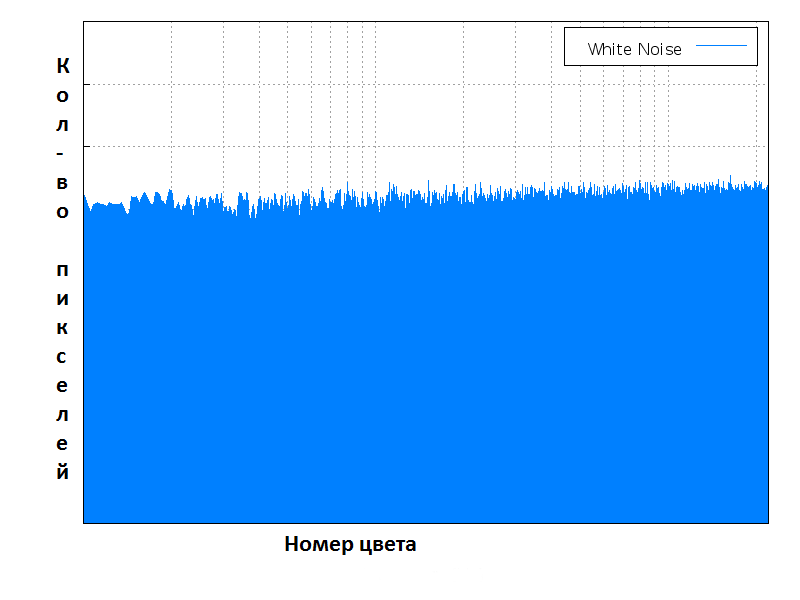
\includegraphics[width=\textwidth]{img/8_white_noise.png}
	\caption{Диаграмма белого шума//почему-то очень много места сверху}
	\label{fig:spire05}
\end{figure}

\subsection{Коричневый шум}
Спектральная плотность коричневого шума пропорциональна 1/f², где f — частота.																									
Это означает, что на низких частотах шум имеет больше энергии, чем на высоких. То есть пикселей темных цветов большей, чем пикселей светлого цвета.Применение фильтра коричневого шума в целом затемняет получаемое изображение.
\\\
\begin{figure}[h]
	\centering
	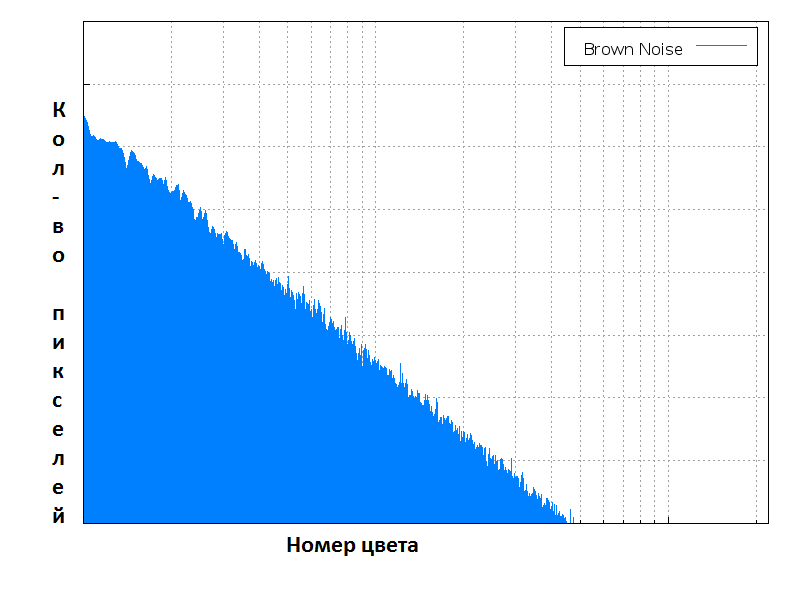
\includegraphics[width=\textwidth ]{img/6_brown_noise.png}
	\caption{Диаграмма красного шума }
	\label{fig:spire04}
\end{figure} 
\begin{lstlisting}[style=pseudocode,caption={Получение коричневого шума}] 
def smoother(noise):
    output = []
    for i in range(len(noise) - 1):
        output.append(0.5 * (noise[i] + noise[i+1]))
return output
\end{lstlisting}

\subsection{Гауссовский шум}

Гауссовский шум  - шум, имеющий функцию плотности вероятности (PDF), равную нормальному распределению, которое также известно как гауссово распределение. 

\begin{equation}
p_g(z)=\frac{1}{\sigma\sqrt{2*\pi}}e^{-\frac{(z-\mu)^2}{2\sigma^2}}
\end{equation}
z - количество цветов, $\mu$ -среднее значение, $\sigma$ - стандартное отклонение.
%\begin{figure}
%	\centering
%  \includegraphics[width=\textwidth]{inc/svg/pic01}
%	\caption{Диаграмма гауссовского шума}
%	\label{fig:spire02}
% \end{figure}
\subsection{Фиолетовый шум}
Фиолетовый  шум представляет собой противооложноть между коричневому шуму. Получение его аналогично получению коричневого шума.Применение фильтра фиолетового шума в целом засветляет получаемое изображение.
\\\\\\\\
\begin{figure}[h!]
	\centering
	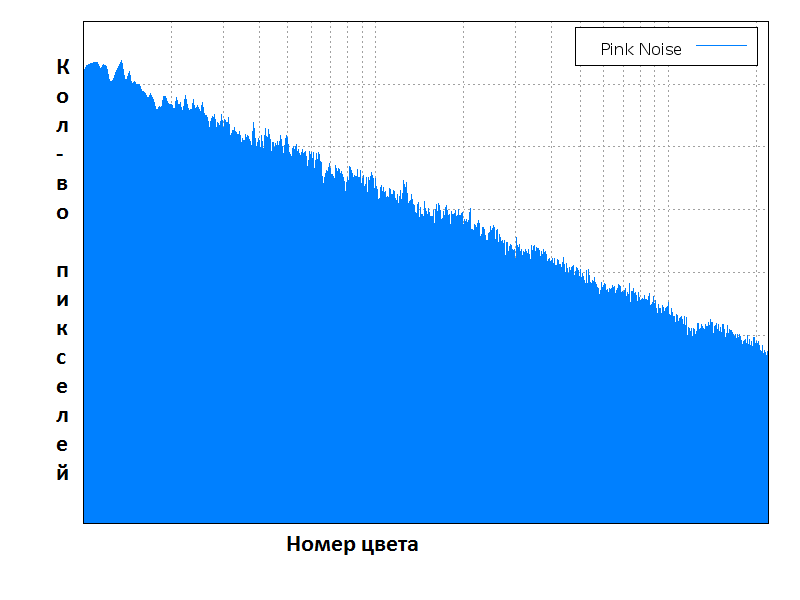
\includegraphics[width=\textwidth]{img/7_pink_noise.png}
	\caption{Диаграмма розового шума}
	\label{fig:spire02}
\end{figure}
\begin{lstlisting}[style=pseudocode,caption={Получение розового шума}]
def rougher(noise):
    output = []
    for i in range(len(noise) - 1):
    output.append(0.5 * (noise[i] - noise[i+1]))
return output
\end{lstlisting}

\subsection{Розовый и синий шумы}
Розовый и синий шумы представляют собой "промежуточные" шумы.Изобржаение с розовым шумом темнее  изображения с белым шумом, но светлее изображения с коричневым шумом. Изображение с синим шумом светлее изображения с белым шумом, но темнее чем изображение с фиолетовым шумом. Их получение аналогично получению со коричневого и фиолетового шумов.

\section{Алгоритм Флойда-Стейнберга}
Рассмотрим более детально алгоритм Флойда-Стейнберга.
P(x,y) - цвет пикселя в точке x,y
I(x,y) - предполгаемый цвет пикселя с учетом ошибки(действительное число)
\begin{figure}[h!]
	\centering
	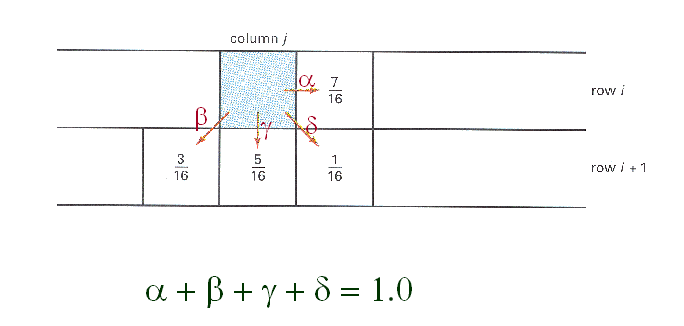
\includegraphics[width=\textwidth]{img/1.png}
	\caption{Схема рассеивания ошибки}
	\label{fig:spire03}
\end{figure}
\begin{lstlisting}[style=pseudocode,caption={Алгоритм Флойда-Стейнберга}]
for x in range(width):
    for y in range(height):
       P(x,y) = trunc(I(x,y)+0.5)
       e = I(x,y) - P(x,y)
       I(x,y+1) += alpha*e
       I(x+1, y-1) += beta*e
       I(x+1, y) += gamma*e
       I(x+1, y+1) += sigma*e
\end{lstlisting}
\section{Комбинация алгоритмов Флойда-Стейнберга и алгоритма случайного распределения}
Комбинируя алгоритмы Флойда-Стейнберга и алгоритм случайнгого распределения, мы, возможно, получим алгоритм, превосходящий их по метрикам SSIM и PSNR.
Идея совмещения заключается в том, что коэффициенты диффузии ошибки вычисляются при помощи генерации элемента последовательти шума. Например, для коэффициента 3/16 и алгоритма белоого шума, можно будет равновероятности получить вместо этого коэффициентв 0/16,1/16,2/16,3/16.\\
Алгоритм комбинации для белого шума, комбинации остальных шумов и алгоритма Флойда-Стейнберга тривиальны и аналогичны. 
\begin{lstlisting}[style=pseudocode,caption={Алгоритм Флойда-Стейнберга и белый шум}]
for x in range(width):
    for y in range(height):
        P(x,y) = trunc(I(x,y)+0.5)
        e = I(x,y) - P(x,y)
        I(x,y+1) += random.randint(1,alpha*16)/16*e
        I(x+1, y-1) += random.randint(1,beta*16)/16*e
        I(x+1, y) += random.randint(1,gamma*16)/16*e
        I(x+1, y+1) +=  random.randint(1,sigma*16)/16*e
\end{lstlisting}


%%% Local Variables:

%%% mode: latex
%%% TeX-master: "rpz"
%%% End:
%--количество цветов
%||количество пикселей
\chapter{Технологический раздел}
\section{Выбор  языка программирования}
Выбранный язык – С++.
Причины:
\begin{enumerate}
	 \item Компилируемый язык со статической типизацией. 
	 \item Сочетание высокоуровневых и низкоуровневых средств.
	 \item Реализация ООП.
	 \item Наличие удобной стандартной библиотеки шаблоны
	 \end{enumerate}
\section{Выбор вспомогательных библиотек}
Для реализации программы была выбрана библиотека Qt.
\begin{enumerate}
	\item Широкие возможности работы с изображениями, в том числе и попиксельно
	\item Наличии более функциональных аналогов стандартной библиотеки шаблонов в том числе для разнообразных структур данных
\end{enumerate}
\subsection{Диаграмма классов}
\begin{figure}[h!]
	\centering
	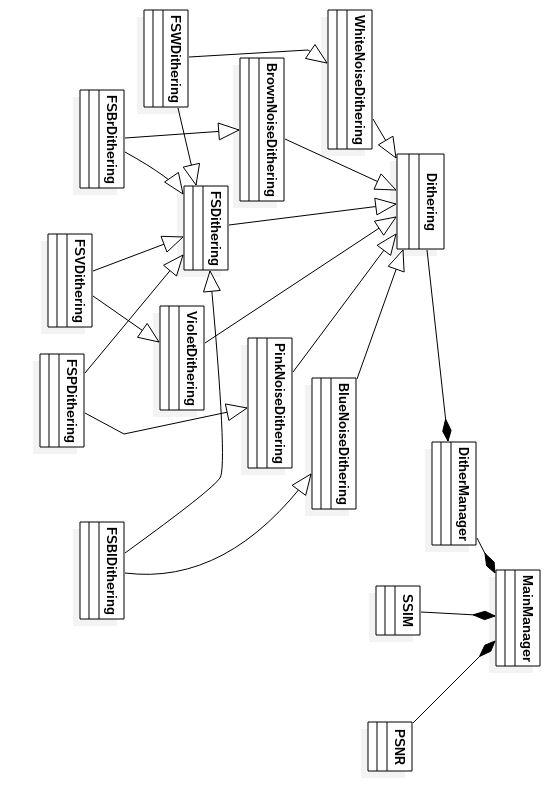
\includegraphics[width=\textwidth]{img/diagramm.png}
	\caption{Диаграмма классов}
	\label{fig:spire03}
\end{figure}

%%% Local Variables:
%%% mode: latex
%%% TeX-master: "rpz"
%%% End:

\chapter{Исследовательский раздел}
%\chapter{Заключение}
\label{cha:research}
\section{Время дизеринга раличных алгоритмов}

%В данном разделе проводятся вычислительные эксперименты.
Рассмотрим время работы различных алгоритмов для различных размеров изображения.
\begin{figure}[h!]
	\centering
	\includegraphics[width=\textwidth]{img/img9.png}
	\caption{Диаграмма времени дизеринга(логарифмическая шкала)}
	\label{fig:spire05}
\end{figure}

\begin{tabular}{|@{\hspace*{2mm}}l||*{3}{c|}}\hline

	&\makebox[12em]{Размер, пиксели}&\makebox[6em]{Время, мкс}
	%	&\makebox[3em]{6/3}&\makebox[3em]{6/4}
	\\\hline\hline
	White noise&133x90&862\\\hline
	Blue noise&133x90&930\\\hline
	Brown noise&133x90&934\\\hline
	Violet noise &133x90&937\\\hline
	Pink noise noise&133x90&930\\\hline
	Floyd-SD&133x90&1200\\\hline
	F. Floyd-SDe&133x90&1093\\\hline
	JJN &133x90&1909\\\hline
	White noise&458x458&15735\\\hline
	Blue noise&458x458&19374\\\hline
	Brown noise&458x458&19432\\\hline
	Violet noise &458x458&18787\\\hline
	Pink noise noise&458x458&18129\\\hline
	Floyd-SD&458x458&27173\\\hline
	F. Floyd-SDe&458x458&26424\\\hline
	JJN &458x458&47201\\\hline
	White noise&458x458&194376\\\hline
	Blue noise&458x458&200577\\\hline
	Brown noise&458x458&208400\\\hline
	Violet noise &458x458&251294\\\hline
	Pink noise noise&458x458&258775\\\hline
	Floyd-SD&458x458&251294\\\hline
	F. Floyd-SDe&458x458&387104\\\hline
	JJN &458x458&857481\\\hline
\end{tabular}
\bigskip
\\
Из рассмотрения вынесены алгоритм Юлиомы в вследствие того, что он значительно медленней других алгоритмов(2732568 мкс для изображения 113х90) в и алгоритм Байера, реализованный при помощи шейдеров, вследствии того, что он не не укладывается в рамки требуемой палитры (при этом он работает очень быстро 64 мс для изображени 640х480).
\section{Качество получаемого изображения}
\begin{tabular}{|@{\hspace*{2mm}}l||*{3}{c|}}\hline
	
	&\makebox[15em]{PSNR}&\makebox[6em]{SSIM}
	%	&\makebox[3em]{6/3}&\makebox[3em]{6/4}
	\\\hline\hline
	White noise&33.2894&0.914778\\\hline
	Blue noise& 36.1756&0.971626\\\hline
	Brown noise&33.32370&0.915767\\\hline
	Violet noise &37.63480&0.984574\\\hline
	Pink noise &36.4484&0.974718\\\hline
	Floyd-SD& 37.0553&0.979173\\\hline
	F. Floyd-SDe&36.8401&0.976452\\\hline
	JJN &37.30740&0.981688\\\hline
	Yliouma&36.2359&0.967796\\\hline
	Without dithering&37.6348&0.984574\\\hline
\end{tabular}
\bigskip
\\
Несмотря на то, что некоторые сложные алгоритмы дизеринга диффузии ошибок обещат получения хорошего качества изображений,некоторые алгоритмы случайного дизеринга на конкретных изображениях дают лучший результат. Для того чтобы получить наилучший результат дизеринга, следует проанализировать результаты дизеринга нескольких изображений и выбрать среди них наилучшее.
Так же следует отметить некоторую необъективность метрик: результат метрик не всегда совпадает с человеческим восприятием картинки.
%\begin{figure}
 % \centering
 % \caption{Как страшно жить}
 % \label{fig:spire01}
%\end{figure}
\section{Размер получаемого изображения}
\begin{figure}[h!]
	\centering
	\includegraphics[width=\textwidth]{img/img10.png}
	\caption{Диаграмма размера изображения(логарифмическая шкала)}
	\label{fig:spire06}
\end{figure}
\begin{tabular}{|@{\hspace*{2mm}}l||*{3}{c|}}\hline
	
	&\makebox[8em]{Разрешение, пикс}&\makebox[5em]{Размер, кб} &\makebox[7em]{Исх. раз., кб}
	%	&\makebox[3em]{6/3}&\makebox[3em]{6/4}
	\\\hline\hline
	White noise&900x675&186&\multirow{6}{*}{2373 bmp,1779 png} \\\cline{1-3}
	Blue noise& 900x675&135& \\\cline{1-3}
	Brown noise&900x6750&186&\\\cline{1-3}
	Violet noise &900x675&98&\\\cline{1-3}
	Pink noise &900x675&1158&\\\cline{1-3}
	Floyd-SD& 900x675&1273&\\\cline{1-3}
	F. Floyd-SDe&900x675&143&\\\cline{1-3}
	JJN &900x675&117&\\\hline
	White noise&3984х32355&3431&\multirow{6}{*}{50344 bmp,37758 png} \\\cline{1-3}
	Blue noise& 3984х3235&2570& \\\cline{1-3}
	Brown noise&3984х3235&3432&\\\cline{1-3}
	Violet noise &3984х3235&1950&\\\cline{1-3}
	Pink noise &3984х3235&2406&\\\cline{1-3}
	Floyd-SD& 3984х32355&3605&\\\cline{1-3}
	F. Floyd-SDe&3984х3235&4269&\\\cline{1-3}
	JJN &3984х3235&3716&\\\hline
\end{tabular}
\bigskip
\\

Из вышеприведенной таблицы, можно заметить, размер изображения после дизеринга значительно уменьшиается,достирается выигрыш в размере изображение до 15 раз, в зависимости от иходного контейнера изображения и выбранного способра дизеринга.
%%% Local Variables:
%%% mode: latex
%%% TeX-master: "rpz"
%%% End:

\chapter{Организационно-экономический раздел}
\label{cha:econom}
%%% Local Variables:
%%% mode: latex
%%% TeX-master: "rpz"
%%% End:

\chapter{Промышленная экология и безопасность}\label{cha:bzd}


%%% Local Variables:
%%% mode: latex
%%% TeX-master: "rpz"
%%% End:


\backmatter %% Здесь заканчивается нумерованная часть документа и начинаются ссылки и
            %% заключение

\Conclusion % заключение к отчёту

\begin{figure}
В данной работе были реализованы различные алгоритмы дизеринга, было произведено сравнение и анализ этих алгоритмов. Программа позволяет получить изображение схожего визуального качества при значительном уменьшении размера. Был получен вывод о том, что для различных целей следует использовать различные алгоритмы дизеринга, универсального алгоритма дизеринга не существует. Программа не привязана к какой-то конкретной
операционной системе и может быть скомпилирована и запущена на
всех популярных ОС.
\end{figure}
%%% Local Variables: 
%%% mode: latex
%%% TeX-master: "rpz"
%%% End: 


% % Список литературы при помощи BibTeX
% Юзать так:
%
% pdflatex rpz
% bibtex rpz
% pdflatex rpz

\bibliographystyle{gost780u}
\bibliography{rpz}


%%% Local Variables: 
%%% mode: latex
%%% TeX-master: "rpz"
%%% End: 


\appendix   % Тут идут приложения

\chapter{Картинки}
\label{cha:appendix1}

\begin{figure}
\centering
\caption{Картинка в приложении. Страшная и ужасная.}
\end{figure}

%%% Local Variables: 
%%% mode: latex
%%% TeX-master: "rpz"
%%% End: 

%\chapter{Еще картинки}
%\label{cha:appendix2}

%\begin{figure}
%\centering
%\caption{Еще одна картинка, ничем не лучше предыдущей. Но %надо же как-то заполнить место.}
%\end{figure}

%%% Local Variables: 
%%% mode: latex
%%% TeX-master: "rpz"
%%% End: 


\end{document}

%%% Local Variables:
%%% mode: latex
%%% TeX-master: t
%%% End:
